\chapter{Stand der Praxis}
\label{ch:StandDerPraxis}

% TODO Historie des betroffenen Feld

In diesem Kapitel werden die gängigen Techniken und Ansätze zur Berechnung von User und Item Nachbarn vorgestellt.

\section{Technologische Grundlagen, Vokabular und Notation}
% TODO Wichtige technologischen Grundlagen / Wissenswertes
In dieser Arbeit wird eine konsistente mathematische Notation verwendet. In Anlehnung an die Notation von \cite{Ekstrand2011} werden deshalb folgende wichtige Elemente zur Berechnung von User zu User Ähnlichkeit und Item zu Item Ähnlichkeit eingeführt. Die wichtigsten Elemente sind die Menge der User $U$ und die Menge der Items $I$. $I_u$ bezeichnet die Menge der Items, welche vom User $u$ bewertet wurden. $U_i$ ist die Menge der User, welche Item $i$ bewertet haben.

Die Ratingmatrix $R$ besteht aus Werten $r_{u,i}$, welche die Bewertungen, welche User $u$ dem Item $i$ gegeben hat, sind. Ein Beispiel wie die Ratingmatrix $R$ aufgebaut ist, zeigt die Tabelle \ref{Ratingmatrix}.
$r_u$ bezeichnet den Vektor aller Ratings von User $u$ (Zeilen von $R$) und Vektor $r_i$ ist der Vektor aller Ratings von Item $i$ (Spalten von $R$).

\begin{table}[htb]
    \caption{Ratingmatrix $R$}
    \label{Ratingmatrix}
    \begin{tabularx}{\textwidth}{|X|X|X|X|X|}
    	\hline 
    	\textbf{} & \textbf{Item 1} & \textbf{Item 2} & \textbf{...}& \textbf{Item n} \\
    	\hline 
    	\textbf{User 1}& $r_{1,1}$ & $r_{1,2}$ & ... & $r_{1,n}$\\ 
    	\hline 
    	\textbf{User 2} &  $r_{2,1}$ & $r_{2,2}$ & ... & $r_{2,n}$\\ 
    	\hline
    	\textbf{...}& ... & ... & ... & ...\\
    	\hline
    	\textbf{User m} &  $r_{m,1}$ & $r_{m,2}$ & ... & $r_{m,n}$\\
    	\hline
    \end{tabularx}
\end{table}


\subsection{Feature Space}
Der Feature Space wird durch die Anzahl Features definiert.
Bei der User zu User Ähnlichkeit betrachtet man die Matrix $R$, sodass jedes Item ein Feature ist. Bei der Item zu Item Ähnlichkeit benützt man zur Berechnung die transponierte Matrix $R^T$, wobei dann die User jeweils die Feature repräsentieren.

%Given some data, a feature space is just the set of all possible values for a chosen set of features from that data. It is always possible to represent feature values and thus a feature space using only numbers, and further to do so in such a way that the feature space can be interpreted as a real space.

\subsection{Principal Component Analysis}
Wenn die Daten eine grosse Anzahl Dimensionen enthalten, kann mittels Principal Component Analysis eine Reduktion der Dimensionen durchgeführt werden.

Die Principal Component Analysis ist definiert als die orthogonale lineare Transformation von Daten, die diese in ein neues Koordinatensystem transformiert. Der Hauptvorteil der Principal Component Analysis besteht darin, dass die Daten so transformiert werden, dass die grösste Varianz durch eine skalare Projektion der Daten auf der ersten Koordinate, dem ersten Principal Component, liegt, die zweitgrösste Varianz auf der zweiten Koordinate, usw. (\cite{jolliffe_principal_2002}, S.28). Dies erlaubt es, die Anzahl der gewünschten Dimensionen zu definieren, ohne zu viele Informationen zu verlieren.

Dies wird mittels Abbildung \ref{fig:PCA} aufgezeigt.

\begin{figure}[ht]
	\centering
	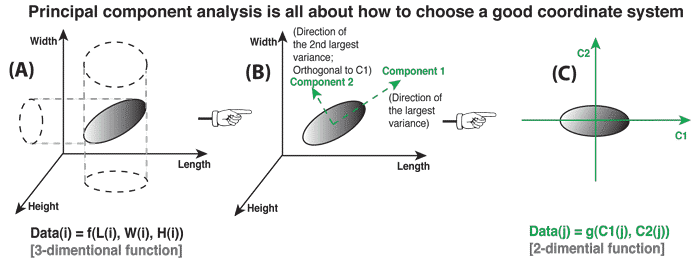
\includegraphics[keepaspectratio,width=0.66\linewidth]{img/PCA.png}
	\caption{Principal Component Analyse, (Quelle: \nameref{sec:Aufgabenstellung}})
	\label{fig:PCA}
\end{figure}

\subsubsection{Berechnung der Principal Component Analyse}
\label{sec: Berechnung PCA}
Es git verschiedene Möglichkeiten um die PCA zu berechnen. Entweder wird die PCA mittels Singulärwertzerlegung  oder mittels Berechnung der Eigenwerte und Eigenvektoren der Daten berechnet. In diesem Abschnitt wird die Berechnung der PCA mit Eigenwerten und -vektoren aufgezeigt. (\cite{principa25:online})


Um die PCA zu berechnen werden im \textbf{ersten} Schritt die vorhandenen Daten in eine $m\times n$ Matrix transformiert (in unserem Fall in die Ratingmatrix $R$). Damit die Principal Component Analysis korrekt funktioniert, subtrahiert man in einem \textbf{zweiten} Schritt in jeder Dimension(Spalten der $m \times n$ Matrix) den Mittelwert $\bar{X}$ der Dimension.  Dadurch erhält man ein Datenset mit dem Mittelwert $= 0$.
Im \textbf{dritten} Schritt berechnet man die $n\times n$ Kovarianzmatrix $C$. Mit der Kovarianzmatrix berechnet man die Kovarianz zwischen allen Dimensionen. Dies wird mit dem Beispiel \eqref{Kovarianzmatrix} mit den drei Dimensionen $X,Y,Z$ aufgezeigt.

\indexequation{C=\left(\begin{array}{ccc}
\operatorname{cov}(x, x) & \operatorname{cov}(x, y) & \operatorname{cov}(x, z) \\
\operatorname{cov}(y, x) & \operatorname{cov}(y, y) & \operatorname{cov}(y, z) \\
\operatorname{cov}(z, x) & \operatorname{cov}(z, y) & \operatorname{cov}(z, z)
\end{array}\right)}{Beispiel einer Kovarianzmatrix mit 3 Dimensionen }{Kovarianzmatrix} 

Wobei man ${cov}(X,Y)$ mit $n$ Dimensionen wie folgt berechnet:
\indexequation{\operatorname{cov}(X, Y)=\frac{\sum_{i=1}^{n}\left(X_{i}-\bar{X}\right)\left(Y_{i}-\bar{Y}\right)}{(n-1)}}{Kovarianz}{Kovarianz}
Da wir im zweiten Schritt bereits den Mittelwert der Dimension substrahiert haben, kann in diesem Fall die Subtraktion von $\bar{X}$ und $\bar{Y}$ weggelassen werden.

Im \textbf{vierten} Schritt werden die Eigenwerte sowie die Eigenvektoren der Kovarianzmatrix $C$ berechnet.
Der Eigenvektor mit dem grössten zugehörigen Eigenwert ist der Principle Component des Datensets. Weiter sortiert man deshalb die Eigenvektoren nach ihren Eigenwerten.
Für die weiteren Schritte, kann man entweder mit allen Eigenvektoren fortfahren, oder man wählt die ersten $n$ Eigenvektoren aus. Dabei kann man auf eine bestimmte Anzahl Dimensionen reduzieren, oder man wählt die Anzahl Eigenvektoren aus, welche $x\%$ der Varianz der Daten enthält.
\subsubsection{PCA Space}
Um nun die Daten im PCA-Space zu erhalten, multiplizieren wir als \textbf{fünfter} und letzter Schritt die transponierten, normierten Daten aus Schritt 2 ($R^T$) mit der transponierten Eigenvektormatrix $E^T$. 
%TODO MUSS FINAL DATA AUCH WIEDER TRANSPONIERT WERDEN? DENKE JA



\subsection{Ähnlichkeitsfunktionen}
Um die User zu User und Item zu Item Ähnlichkeit zu berechnen, kommen unterschiedliche Ähnlichkeitsfunktionen in Frage. In diesem Subkapitel werden drei Ähnlichkeitsfunktionen vorgestellt.

\subsubsection{Pearson Korrelation}
Die Pearson Korellation ermittelt die statistische Korrelation zweier Variabeln und wird auch von Grouplens (\cite{Resnick94grouplens:an}) zur Ermittlung der User zu User Ähnlichkeit verwendet. Der Pearson-Korrelationskoeffizient kann Werte zwischen $-1$ und $1$ annehmen und wird wie folgt berechnet:

\indexequation{s(u, v)=\frac{\sum_{i \in I_{u} \cap I_{v}}\left(r_{u, i}-\bar{r}_{u}\right)\left(r_{v, i}-\bar{r}_{v}\right)}{\sqrt{\sum_{i \in I_{u} \cap_{v}}\left(r_{u, i}-\bar{r}_{u}\right)^{2}} \sqrt{\sum_{i \in I_{u} \cap_{v}}\left(r_{v, i}-\bar{r}_{v}\right)^{2}}}}{Pearson Korrelation}{Pearson Korrelation}



\subsubsection{Cosinus Similarität}

Die Cosinus Similarität ist, anderst als die Pearson Korrelation, kein statistischer Ansatz sondern vielmehr ein auf der linearen Algebra basierender Ansatz um die Ähnlichkeit zwischen zwei User oder zwei Items zu berechnen. Dazu werden jeweils die Ratingvektoren $r_u$ für die User und die Ratingvektoren $r_i$ für die Items verwendet.
Mit $r_u$ beziehungsweise $r_i$ wird die Cosinus Distanz berechnet. Dazu wird das Skalarprodukt zwischen $r_u$ und $r_v$ für die Items $r_i$ und $r_j$ berechnet und durch ihre $L_2$ Norm geteilt.
Folgend die Formeln für die Cosinus Similarität jeweils mit $r_u$,$r_v$ für die User und mit $r_i$,$r_j$ für die Item (\cite{Ekstrand2011}).

\indexequation{s(u, v)=\frac{\mathbf{r}_{u} \cdot \mathbf{r}_{v}}{\left\|\mathbf{r}_{u}\right\|_{2}\left\|\mathbf{r}_{v}\right\|_{2}}=\frac{\sum_{i} r_{u, i} r_{v, i}}{\sqrt{\sum_{i} r_{u, i}^{2}} \sqrt{\sum_{i} r_{v, i}^{2}}}}{Cosinus Similarität User $u,v$}{Cosinus Similarität User $u,v$}

\indexequation{s(i, j)=\frac{\mathbf{r}_{i} \cdot \mathbf{r}_{j}}{\left\|\mathbf{r}_{i}\right\|_{2}\left\|\mathbf{r}_{j}\right\|_{2}}}{Cosinus Similarität Item $i,j$}{Cosinus Similarität Item $i,j$}


\subsubsection{Mahalanobis Distanz}
Die Mahalanobis Distanz wurde 1936 von P.C. Mahalanobis eingeführt (\cite{mahalanobis1936generalized}).
Die Mahalonobis Distanz wird definiert als (\cite{DEMAESSCHALCK20001}):
\indexequation{$$\mathrm{MD}_{u}=\sqrt{\left(r_{u}-\bar{r}\right) \mathrm{C}^{-1}\left(r_{u}-\bar{r}\right)^{T}}$$}{Mahalanobis Distanz}{Mahalanobis Distanz}

Wobei $C^{-1}$ das Inverse der Covarianzmatrix C aus Formel  \ref{Kovarianzmatrix} ist.

Soll nun die Mahalanobis Distanz zwischen zwei Vektoren berechnet werden, so kann der Mittelwert $\bar{r}$ in Formel \ref{Mahalanobis Distanz} durch einen Zweiten Vektor ausgetauscht werden. So kann Formel \ref{Mahalanobis Distanz} geschrieben werden als Mahalanobis Distanz zwischen zwei User:

\indexequation{$$\mathrm{MD}_{u,m}=\sqrt{\left(r_{u}-r_{m}\right) \mathrm{C}^{-1}\left(r_{u}-r_{m}\right)^{T}}$$}{Mahalanobis Distanz zwischen zwei User}{Mahalanobis Distanz mit zwei User}

Beziehungsweise als Mahalanobis Distanz zwischen zwei Items:

\indexequation{$$\mathrm{MD}_{i,n}=\sqrt{\left(r_{i}-r_{n}\right) \mathrm{C}^{-1}\left(r_{i}-r_{n}\right)^{T}}$$}{Mahalanobis Distanz zwischen zwei Items}{Mahalanobis Distanz mit zwei Items}


\subsection{Vergleich zweier Listen}
Um die Ähnlichkeit der Top $N$ User- beziehungsweise Item-Nachbaren des Feature Space mit den Top $N$ Nachbaren des PCA Spaces zu vergleichen gibt es viele Ansätze. In den folgenden Subkapiteln werden die gängigsten Koeffizienten beschrieben. 
\subsubsection{Jaccard Index}
Der Jaccard Index (\cite{Jaccard}) ist ein in vielen Gebieten, beispielsweise Machine Learning, angewandter Index, um die Ähnlichkeit zweier finiten Mengen zu vergleichen. (\cite{kotz_balakrishnan_vidakovic_campbell}). Der Jaccard Index wird definiert als: \indexequation{$$J(A, B)=\frac{|A \cap B|}{|A \cup B|}=\frac{|A \cap B|}{|A|+|B|-|A \cap B|}$$}{Jaccard Index}{Jaccard Index}


\subsubsection{Tanimoto Koeffizient}
Der Tanimoto Koeffizient ist eine Erweiterung des Jaccard Index. Da der Jaccard Index nur überprüft, ob ein Item oder User $\in$ der Mengen $A,B$ ist.
Der Tanimoto Koeffizient erweitert den Jaccard Index so, dass nicht nur überprüft wird, ob die Items und User in den Mengen $A,B$ vorhanden sind, sondern die Mengen $A$ und $B$ werden elementweise miteinander verglichen.

Der Tanimoto Koeffizient wird wie folgt definiert (\cite{Rogers1960}):
\indexequation{$$T_{s}(A, B)=\frac{\sum_{i}\left(A_{i} \wedge B_{i}\right)}{\sum_{i}\left(A_{i} \vee B_{i}\right)}$$}{Tanimoto Koeffizient}{Tanimoto Koeffizient}
